\documentclass[12pt,a4paper]{article}
\usepackage{geometry} % Required for adjusting page dimensions and margins
\geometry{
	paper=a4paper, % Paper size, change to letterpaper for US letter size
	top=2.5cm, % Top margin
	bottom=3cm, % Bottom margin
	left=2.5cm, % Left margin
	right=2.5cm, % Right margin
	headheight=14pt, % Header height
	footskip=1.5cm, % Space from the bottom margin to the baseline of the footer
	headsep=1.2cm, % Space from the top margin to the baseline of the header
	%showframe, % Uncomment to show how the type block is set on the page
}
\usepackage{amsmath,amsfonts,stmaryrd,amssymb} % Math packages
\usepackage{wrapfig}
\usepackage{graphicx}
\usepackage{mathtools}
\usepackage{subcaption}
\usepackage{listings}
\usepackage[ruled]{algorithm2e} % Algorithms
\usepackage{listings} % File listings, with syntax highlighting
\lstset{
	basicstyle=\ttfamily, % Typeset listings in monospace font
}
\usepackage{enumerate} % Custom item numbers for enumerations
\usepackage[framemethod=tikz]{mdframed} % Allows defining custom boxed/framed environments
\usepackage{url}
\usepackage{hyperref}
\usepackage{xcolor}
\usepackage{fancyhdr}
\pagestyle{fancy}
\fancyhf{}
\usepackage[utf8]{inputenc} % Required for inputting international characters
\usepackage[T1]{fontenc} % Output font encoding for international characters

\usepackage{XCharter} % Use the XCharter fonts
%----------------------------------------------------------------------------------------
%	COMMAND LINE ENVIRONMENT
%----------------------------------------------------------------------------------------

% Usage:
% \begin{commandline}
%	\begin{verbatim}
%		$ ls
%		
%		Applications	Desktop	...
%	\end{verbatim}
% \end{commandline}

\mdfdefinestyle{commandline}{
	leftmargin=10pt,
	rightmargin=10pt,
	innerleftmargin=15pt,
	middlelinecolor=black!50!white,
	middlelinewidth=2pt,
	frametitlerule=false,
	backgroundcolor=black!5!white,
	frametitle={Command Line},
	frametitlefont={\normalfont\sffamily\color{white}\hspace{-1em}},
	frametitlebackgroundcolor=black!50!white,
	nobreak,
}

% Define a custom environment for command-line snapshots
\newenvironment{commandline}{
	\medskip
	\begin{mdframed}[style=commandline]
	}{
	\end{mdframed}
	\medskip
}

%----------------------------------------------------------------------------------------
%	FILE CONTENTS ENVIRONMENT
%----------------------------------------------------------------------------------------

% Usage:
% \begin{file}[optional filename, defaults to "File"]
%	File contents, for example, with a listings environment
% \end{file}

\mdfdefinestyle{file}{
	innertopmargin=1.6\baselineskip,
	innerbottommargin=0.8\baselineskip,
	topline=false, bottomline=false,
	leftline=false, rightline=false,
	leftmargin=2cm,
	rightmargin=2cm,
	singleextra={%
		\draw[fill=black!10!white](P)++(0,-1.2em)rectangle(P-|O);
		\node[anchor=north west]
		at(P-|O){\ttfamily\mdfilename};
		%
		\def\l{3em}
		\draw(O-|P)++(-\l,0)--++(\l,\l)--(P)--(P-|O)--(O)--cycle;
		\draw(O-|P)++(-\l,0)--++(0,\l)--++(\l,0);
	},
	nobreak,
}

% Define a custom environment for file contents
\newenvironment{file}[1][File]{ % Set the default filename to "File"
	\medskip
	\newcommand{\mdfilename}{#1}
	\begin{mdframed}[style=file]
	}{
	\end{mdframed}
	\medskip
}

%----------------------------------------------------------------------------------------
%	NUMBERED QUESTIONS ENVIRONMENT
%----------------------------------------------------------------------------------------

% Usage:
% \begin{question}[optional title]
%	Question contents
% \end{question}

\mdfdefinestyle{question}{
	innertopmargin=1.2\baselineskip,
	innerbottommargin=0.8\baselineskip,
	roundcorner=5pt,
	nobreak,
	singleextra={%
		\draw(P-|O)node[xshift=1em,anchor=west,fill=white,draw,rounded corners=5pt]{%
			Question \theQuestion\questionTitle};
	},
}

\newcounter{Question} % Stores the current question number that gets iterated with each new question

% Define a custom environment for numbered questions
\newenvironment{question}[1][\unskip]{
	\bigskip
	\stepcounter{Question}
	\newcommand{\questionTitle}{~#1}
	\begin{mdframed}[style=question]
	}{
	\end{mdframed}
	\medskip
}
%----------------------------------------------------------------------------------------
%	WARNING TEXT ENVIRONMENT
%----------------------------------------------------------------------------------------

% Usage:
% \begin{warn}[optional title, defaults to "Warning:"]
%	Contents
% \end{warn}

\mdfdefinestyle{warning}{
	topline=false, bottomline=false,
	leftline=false, rightline=false,
	nobreak,
	singleextra={%
		\draw(P-|O)++(-0.5em,0)node(tmp1){};
		\draw(P-|O)++(0.5em,0)node(tmp2){};
		\fill[black,rotate around={45:(P-|O)}](tmp1)rectangle(tmp2);
		\node at(P-|O){\color{white}\scriptsize\bf !};
		\draw[very thick](P-|O)++(0,-1em)--(O);%--(O-|P);
	}
}

% Define a custom environment for warning text
\newenvironment{warn}[1][Warning:]{ % Set the default warning to "Warning:"
	\medskip
	\begin{mdframed}[style=warning]
		\noindent{\textbf{#1}}
	}{
	\end{mdframed}
}

%----------------------------------------------------------------------------------------
%	INFORMATION ENVIRONMENT
%----------------------------------------------------------------------------------------

% Usage:
% \begin{info}[optional title, defaults to "Info:"]
% 	contents
% 	\end{info}

\mdfdefinestyle{info}{%
	topline=false, bottomline=false,
	leftline=false, rightline=false,
	nobreak,
	singleextra={%
		\fill[black](P-|O)circle[radius=0.4em];
		\node at(P-|O){\color{white}\scriptsize\bf i};
		\draw[very thick](P-|O)++(0,-0.8em)--(O);%--(O-|P);
	}
}

% Define a custom environment for information
\newenvironment{info}[1][Problem Statement:]{ % Set the default title to "Info:"
	\medskip
	\begin{mdframed}[style=info]
		\noindent{\textbf{#1}}
	}{
	\end{mdframed}
}



\hypersetup{colorlinks=true,linkcolor=cyan,citecolor=cyan,urlcolor=cyan}


%\fancyhead[LE,RO]{Raspberry Pi}
\fancyhead[RE,LO]{Wireless Ordering \& Billing System for Restaurants}
%\fancyfoot[CE,CO]{\leftmark}
\fancyfoot[CE,CO]{\thepage}
\renewcommand{\headrulewidth}{2pt}
\renewcommand{\footrulewidth}{1pt}

\author{\textbf{Anshuman Singh} \\ \textbf{2018JTM2004}\\ \textbf{2018-19}}
\date{}
\title{\textbf{ELP - 720 Telecom Networks Laboratory}}

\begin{document}
	\maketitle
	
	\begin{center}
	\noindent \textbf{\large A report presented on}\\
	\Huge \textbf{Wireless Ordering \& Billing System for Restaurants} 
	\vspace{1cm}
	
	\begin{figure}[h]
	\centering
	
\includegraphics[scale=.2]{iitd.jpg}
	
	
	\end{figure}
	\vspace{1.5cm}
	
	\textbf{\Large Bharti School\\of\\Telecommunication Technology and Management\\IIT DELHI, Delhi\\ \today}
	
	\end{center}
	
	\newpage
	\tableofcontents
	\listoffigures
	\newpage
	
	\section{Introduction}
	\begin{info}[Problem Statement]Many times in hotel we have to wait for a waiter to give our order for food. This creates
	problem when there is rush in hotel especially in festival seasons and generally on
	weekends. Also, there are self-service hotels where customers have to get up each
	time to place and receive their orders. Customers also expect to have an idea about
	service time and total bill beforehand. Main intention of our project is to avoid such
	problems and to give a cost effective solution to such problems.
	\end{info}	
	\begin{info}[Proposed Solution]
	The project is based on client-server model where the customer sitting at a table is the
	client and the chef or employees of the restaurant will act as server. The user will be
	presented with a paper based menu along with a few buttons and an LCD panel. The
	paper based menu will be modular in terms of Menu Card attached which can be
	changed/updated by just changing the card. Next to menu items there will be buttons
	to choose an item on a particular page. Since items are distributed on a number of
	pages and only few buttons are available to make selections, there will a mechanism
	available to determine which page user is on. Depending on the page opened,
	pressing a button next to a menu item will select the item on that particular page and
	show the same on LCD below. A seven segment display can be attached next to each
	Button to display count of selections made corresponding to each page. After
	choosing the menu items order can be placed using a button. This order will be sent
	through Wi-Fi to the server which is a computer running a server. The Server side will
	do all the processing on order and send an appropriate message which will be
	displayed on LCD. At the end when user requests the Bill the same can be displayed
	on LCD.
	\end{info}
		
		\section{Project Architecture}
		In total, project consist of a micro-controller (ESP32), a 20*4 LCD, few buttons, 7 segment displays, LDRs, resistors and a paper menu card all put together on a single board. The menu card has a predefined format in which different menu items are listed in different rows. The menu items on a single page could vary from 8 to greater than 50. In between the pages LDRs have been embedded. For every page turned on, a different set of LDRs get exposed to light. To keep the detection of page accurate paper chosen be thick and dark-coloured. Also, an extra LDR has been placed outside the menu card to act as reference for different lightening conditions. Next to each menu item a button is available to select the corresponding item. 
		
		Below the menu card exists a 20*4 LCD display to show each input given and response received from server. Next to the LCD, exists button to configure the order like placing an order, resetting the selections made and making requests for bill. Users can turn through the pages, choose an item, select it and place an order for the same. Since there are limited buttons and many menu items arranged on different pages LDR circuit determines which page user is on. All of the above items are connected with different GPIOs of ESP-32 which is a wifi based micro-controller. 
		\begin{figure}[h]
			\centering
			\caption{Proposed Layout of Project}
			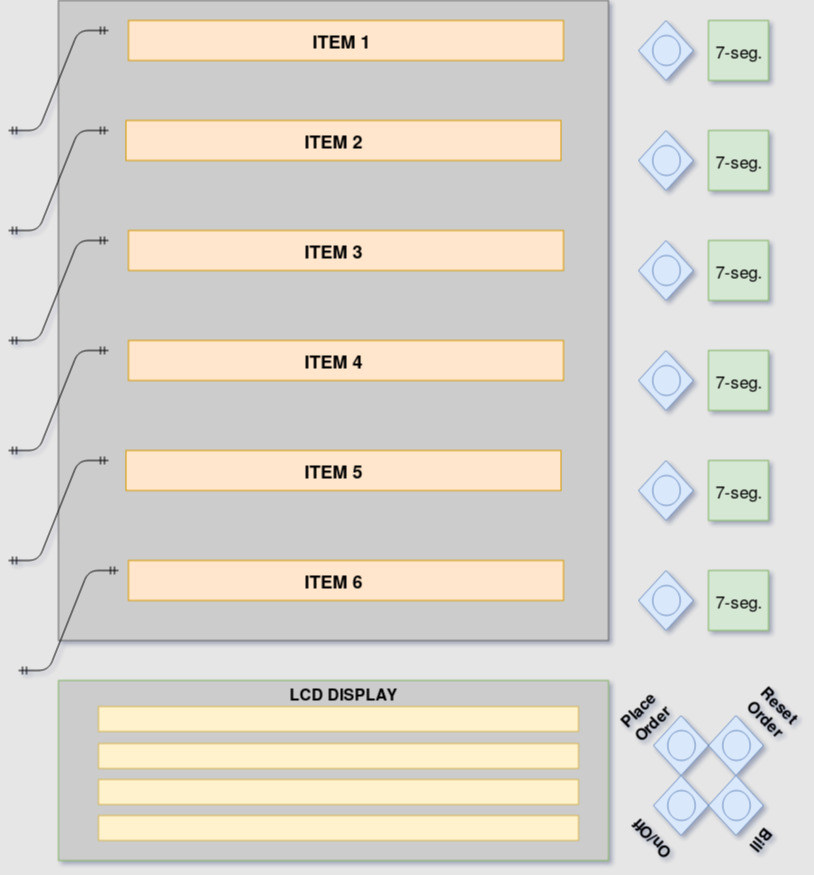
\includegraphics[scale=.5]{layout}
		\end{figure}
		
		ESP32 acts as a client for a python server running on a computer. For every input to the system it sends corresponding requests to server. The communication between the client and server is through a TCP socket. Server running on computer when turned on starts listening for incoming connections from different tables each with its own menu card. Unique identification ID of each ESP32 helps to identify the incoming request. The server makes use of MySQL database to store the request, response, details of every item available along with price and quantity. For different restaurants a different configuration file can be loaded into the MySQL database.
        
        \section{Implementation (Tools and Technologies)}
        The implementation of the project can be divided into the following parts
        \begin{info}[Socket based Client Server Architecture]
        Sockets allow communication between two different processes on the same or different machines. To be more precise, it's a way to talk to other devices using standard Unix file descriptors. Although different types of sockets are available like Stream Sockets, Datagram Sockets, Raw Sockets etc., Stream socket has been used to establish a connection with server as delivery in a networked environment is guaranteed. They use TCP (Transmission Control Protocol) for data transmission. If delivery is impossible, the sender receives an error indicator. Data records do not have any boundaries.
        
        ESP32 when turned on establishes a connection with the pre-fixed network using its SSID and passphrase. Once connected to network it establishes a socket connection with the server using server's IP address and port number.
		\end{info}	
		\begin{info}[I2C protocol to communicate with LCD]
		An I2C protocol is one of the serial communication protocol that is used for the chip to chip communication. The I2C is the short form of Inter-Integrated Circuit, is a type of bus, which designed and developed by Philips in 1980 for inter-chip communication. I2C is basically two-wire communication protocol.It uses only two wire for the communication. In which one wire is used for the data (SDA) and other wire is used for the clock (SCL).
		
		As the number of GPIOs on ESP32 are limited an I2C adapter has been used to communicate with the LCD display with only two pins namely SDA (Data) and SCL (Clock).
		\end{info}
		\begin{info}[Voltage Divider Circuit]
			A voltage divider circuit has been made using resistors. This voltage value is then read using an analog pin of ESP32. When a button is pressed the voltage drop changes. This change in analog pin reading determines which button is pressed. Four buttons can be safely placed on one analog with a sufficient margin to avoid any errors.
		\end{info}
		\begin{info}[Light Dependent Resistors]
		LDR is a component whose light intensity changes as light falls upon it. This property of LDR has been used here in the project. As the intensity of light falling on LDR changes the resistance offered by the LDR changes. Higher the ight intensity falling on LDR lesser the resistance it offers. 
		
		LDR's are placed withing the menu card in a way that at each page turn a different set of LDR's get exposed.
		\end{info}
		\section{Implementation}
		The entire project can be broadly divided into the following sections:
		\begin{info}[Determining Page Number]
		As the menu items are distributed over a few pages and only limited buttons are available to the user, a mechanism based on LDR's to determine the page number is proposed. LDR is a component whose light intensity changes as light falls upon it. This property of LDR has been used here in the project. In the proposed model 4 LDR's have been used in total. One LDR is always exposed to light and determines the current lightening conditions. Three other LDR's are embedded in the menu and a different set of LDR gets exposed as pages are turned. Readings of all these LDR are then compared with the reference LDR to find the page number.
		
		\end{info}
		\begin{info}[Getting user input from buttons]
		There are limited number of GPIO's in ESP32. However a minimum of 10 user inputs for different options needs to be taken. To solve this problem analog pins have been used to get status of buttons. The buttons are connected with a voltage divider circuit with the help of resistors. When a button is pressed the potenial drop changes and this is read through the analog pins of ESp32. A total of 4 buttons have been connected to a single analog pins. This way only 3 analog pins have used to get inputs from all the buttons.
		
		\end{info}
		\begin{info}[Displaying User Input and Server Response]
		To make the interface available to the user more intuitive, a 7 segment display has been placed next to each button which displays the number of items ordered for that menu item. As the page is turned this display gets updated to show  the selections made in that page. Also, a 20*4 LCD has been placed at the bottom of the menu to display the selections made and response from the server. Out of the 4 rows the first row shows the response from server. The middle two rows shows the selection made and user input. The last displays the current status of selections. This gets dynamically updated after a particular time instant as specified in the code.
		\end{info}
		\begin{info}[Connecting with Server]
		Server in this project is a Python Socket Server running on a computer and client is the ESP32 placed on the menu card. When the menu card is turned on ESP32 establishes a connection with Server after connecting to the same network. Here, Server uses a socket connection to communicate with the ESP32 using TCP protocol. For every selection made a request is sent to the server and the response received is shown on the LCD's 1st row.
		
		\end{info}
		
		\begin{info}[Storing Data and Configuration]
		To store the data about available items, past orders, current orders and configuration files MySQL database server has been used. When menu card has to be changed a new configuration file specifying page number, item number and item id can be sourced into MySQL database. To keep records a total of 5 tables in SQL have been used. One table named "available" keeps record of available items, quantity and price uniquely identifiable by their item id's. Next, a table "config" is used for configuring menu card. To keep selections made by ddifferent tables another table named "temp" is used. Another two tables namely "current orders" and "past orders" maintains record of orders placed and billed.
		\end{info}
	    \section{Bill of Materials}
	    \begin{center}
		    \begin{tabular}{|c|c|c|}
		    	\hline
		    	\textbf{Item Name} & \textbf{Quantity} & \textbf{Price (Rs.)} \\
		    	\hline
		    	ESP32 & 1 & 480\\
		    	\hline
		    	LCD 20*4 & 1 & 400\\
		    	\hline
		    	7 segment & 6 & 54\\
		    	\hline
		    	LDRs & 4 & 32\\
		    	\hline
		    	Others & - & 50\\
		    	\hline
		    	\textbf{Total} & -- & \textbf{1016}\\
		    	\hline
			\end{tabular}

	    \end{center}
	    
	    \section{Proposed Milestones and timeline of milestones achieved}
   		\begin{figure}[h]
			\centering
			\caption{Proposed Milestones and timeline of milestones achieved}
			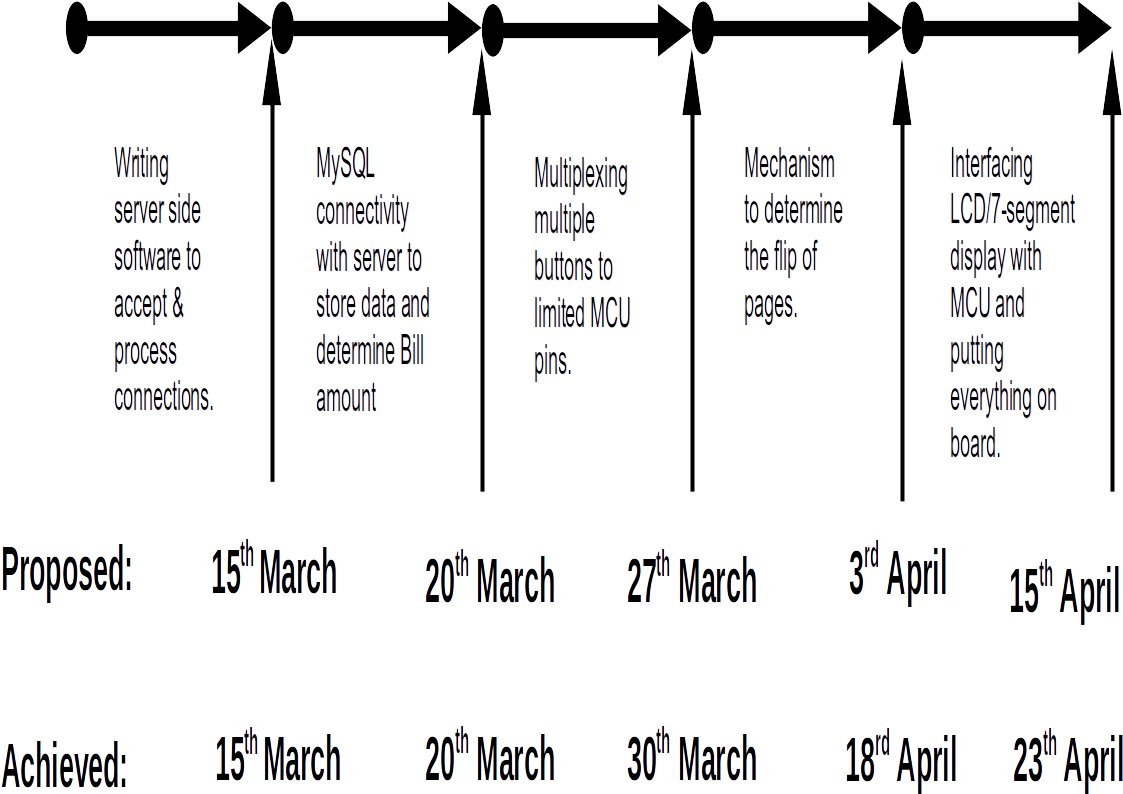
\includegraphics[scale=.45]{timeline}
		\end{figure}

		\newpage
	    \section{Results}
	    \subsection{Overall Final Layout and Architecture}
	    \begin{figure}[h]
	    	\centering
	    	\caption{Final External View of Project}
	    	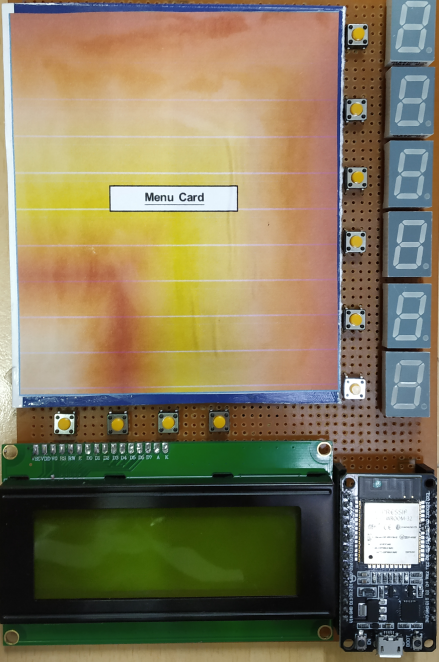
\includegraphics[scale=.7]{overall_layout}
	    \end{figure}
	   \newpage
    	\subsection{User Input and Server Response on LCD}
	\begin{figure}[h]
		\centering
		\begin{subfigure}{.5\textwidth}
			\centering
			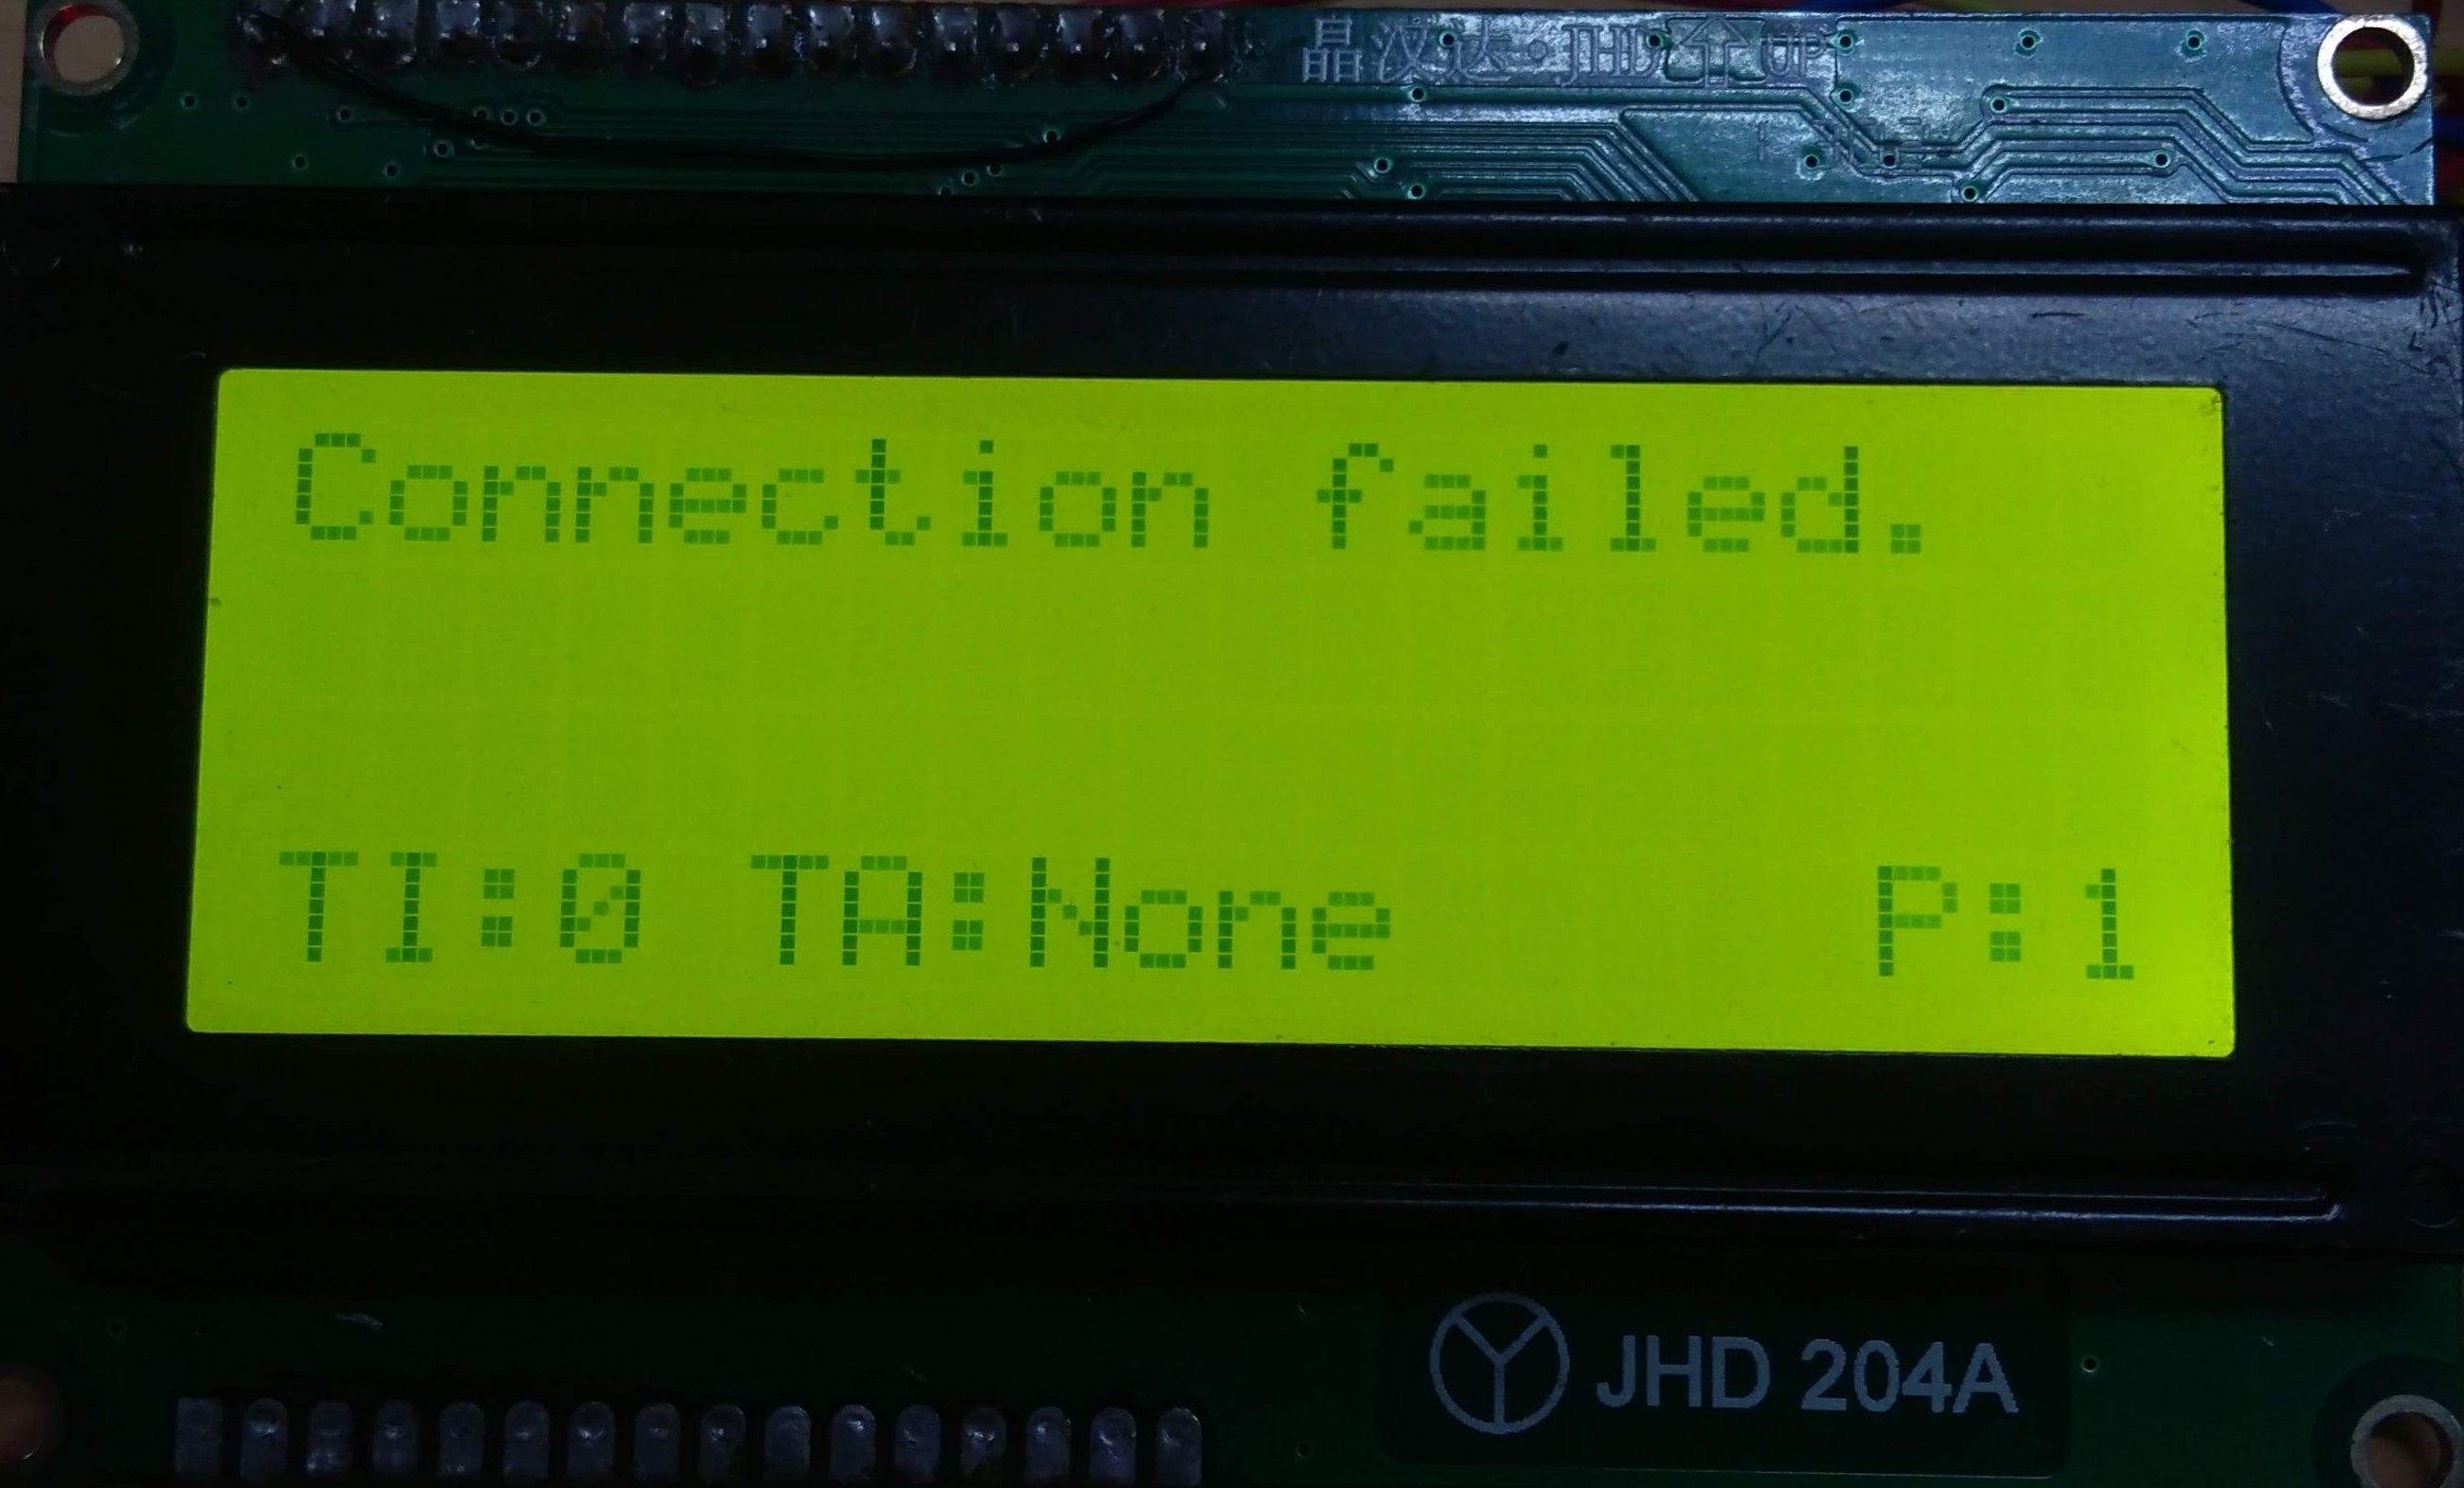
\includegraphics[width=1\textwidth]{con_failed}
		\end{subfigure}%
		\begin{subfigure}{.5\textwidth}
			\centering
			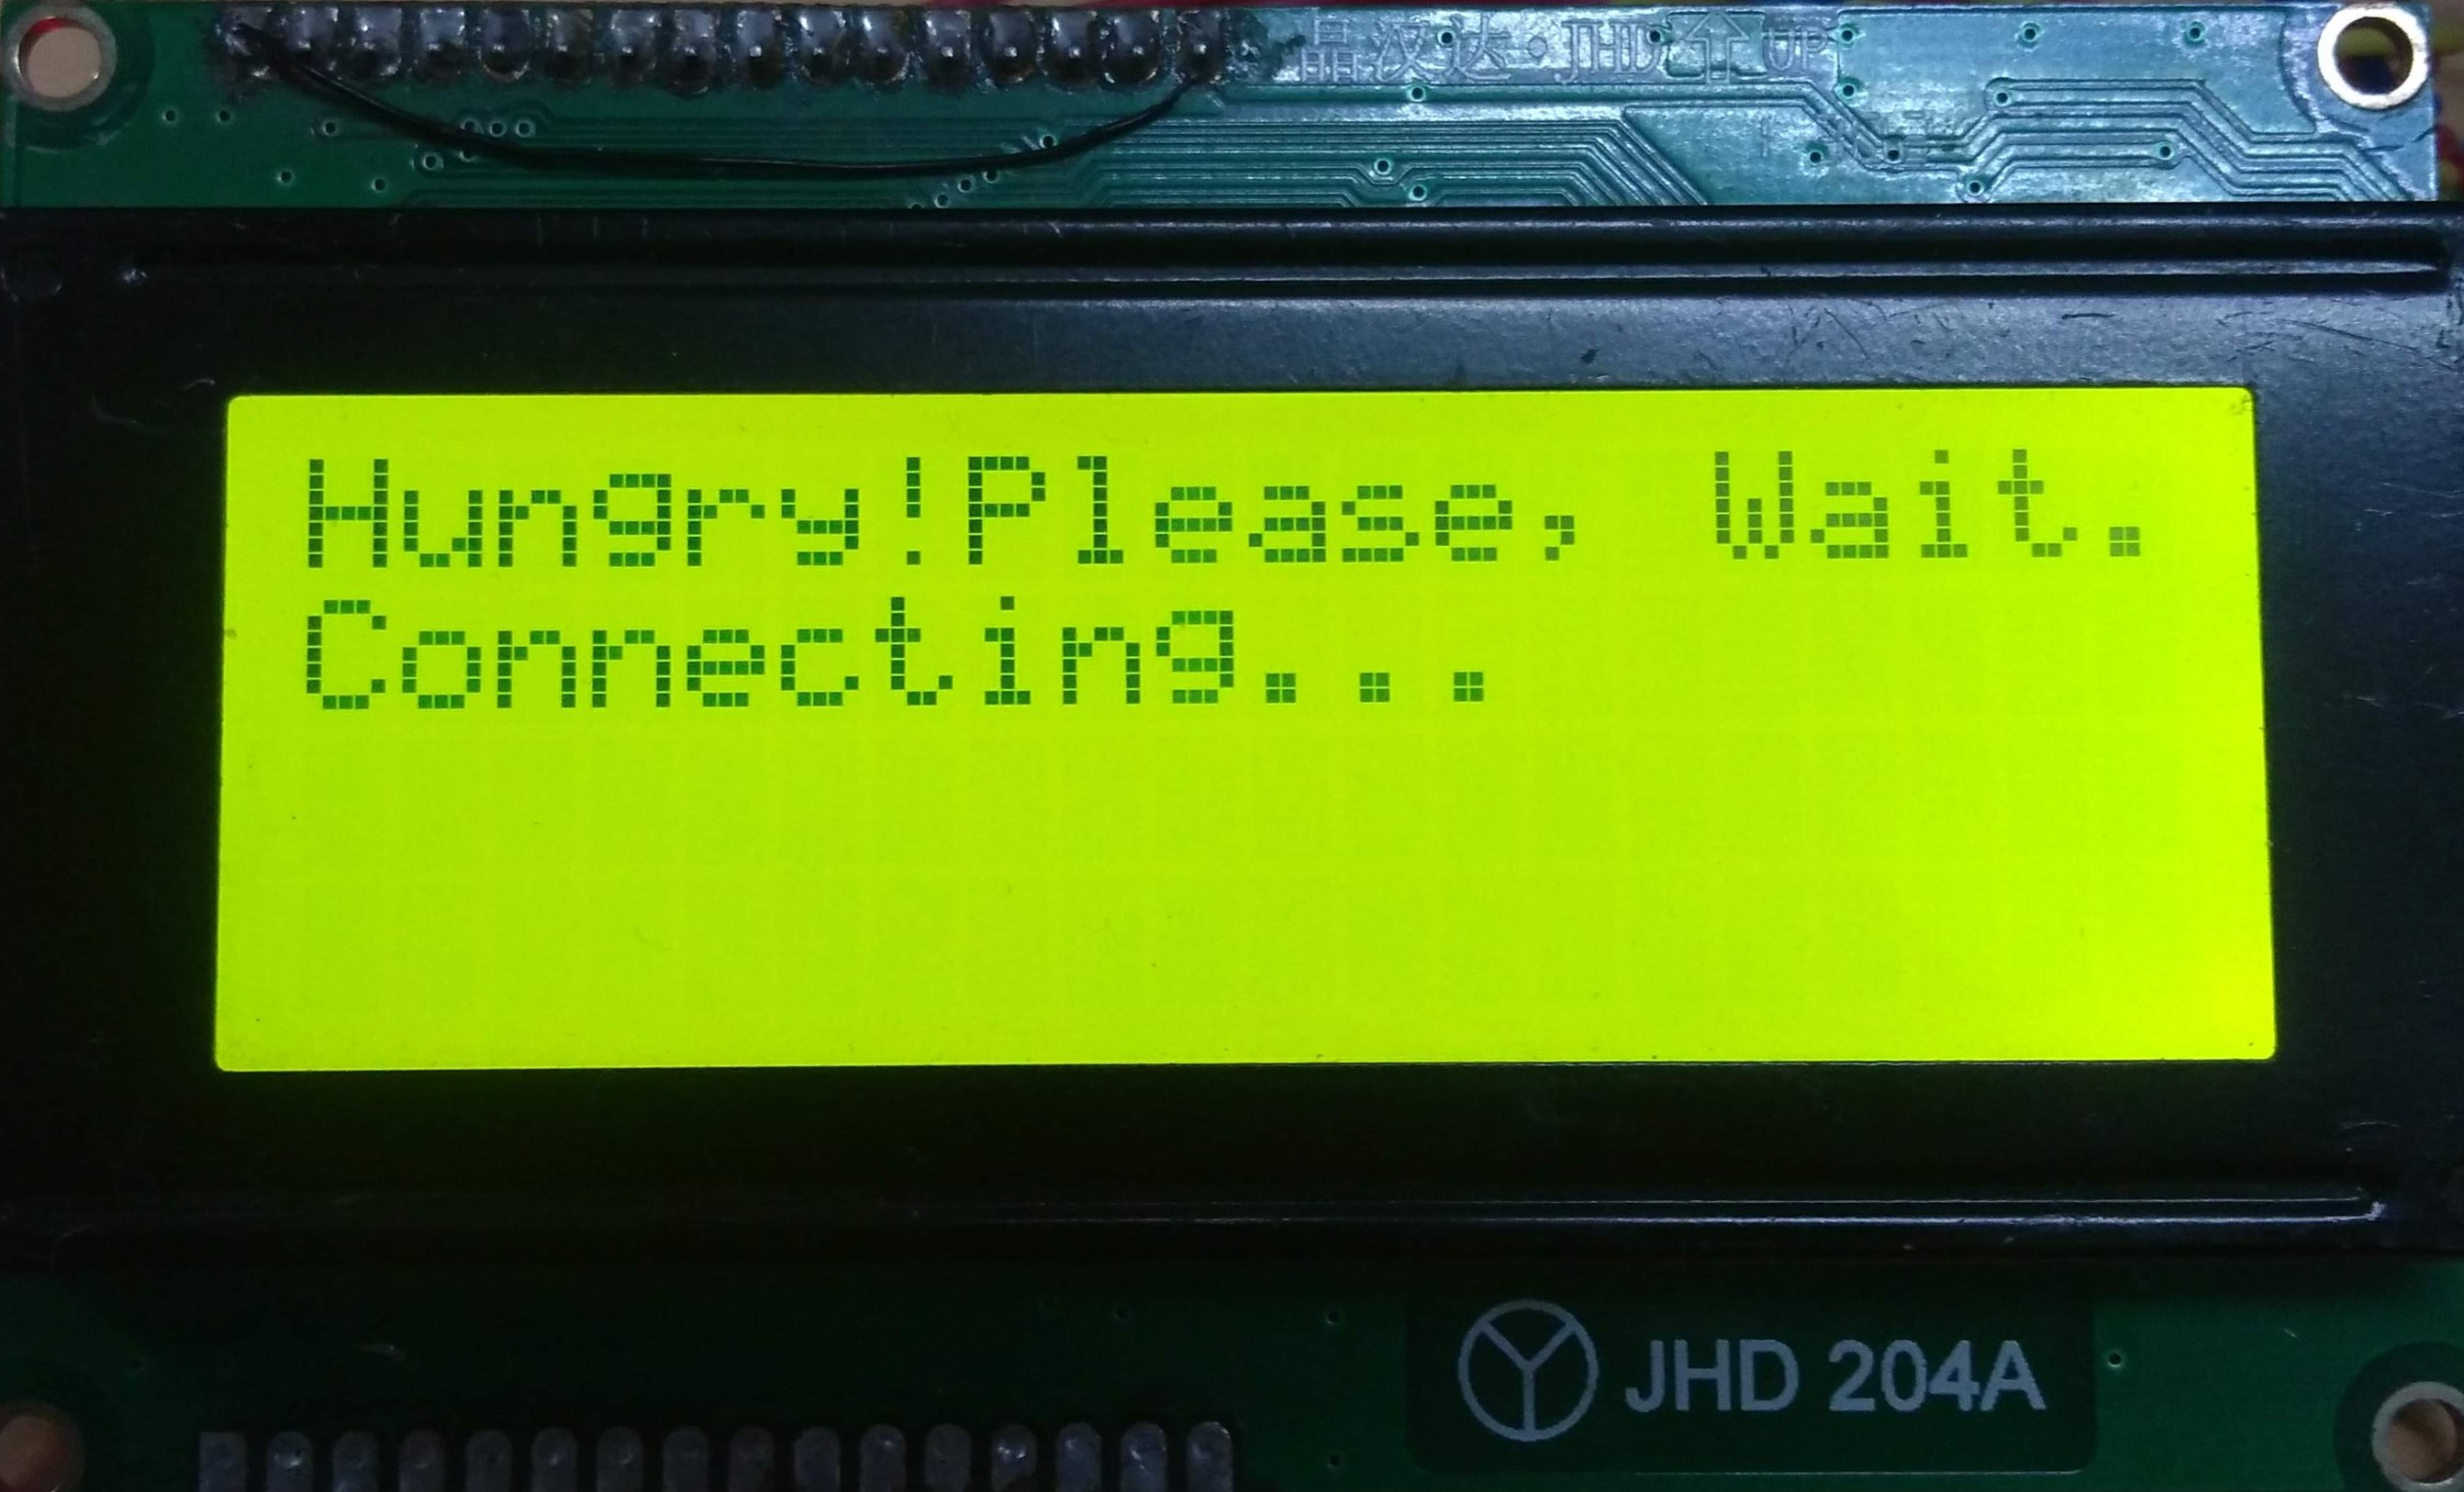
\includegraphics[width=1\textwidth]{entry}
		\end{subfigure}
		\begin{subfigure}{.5\textwidth}
			\centering
			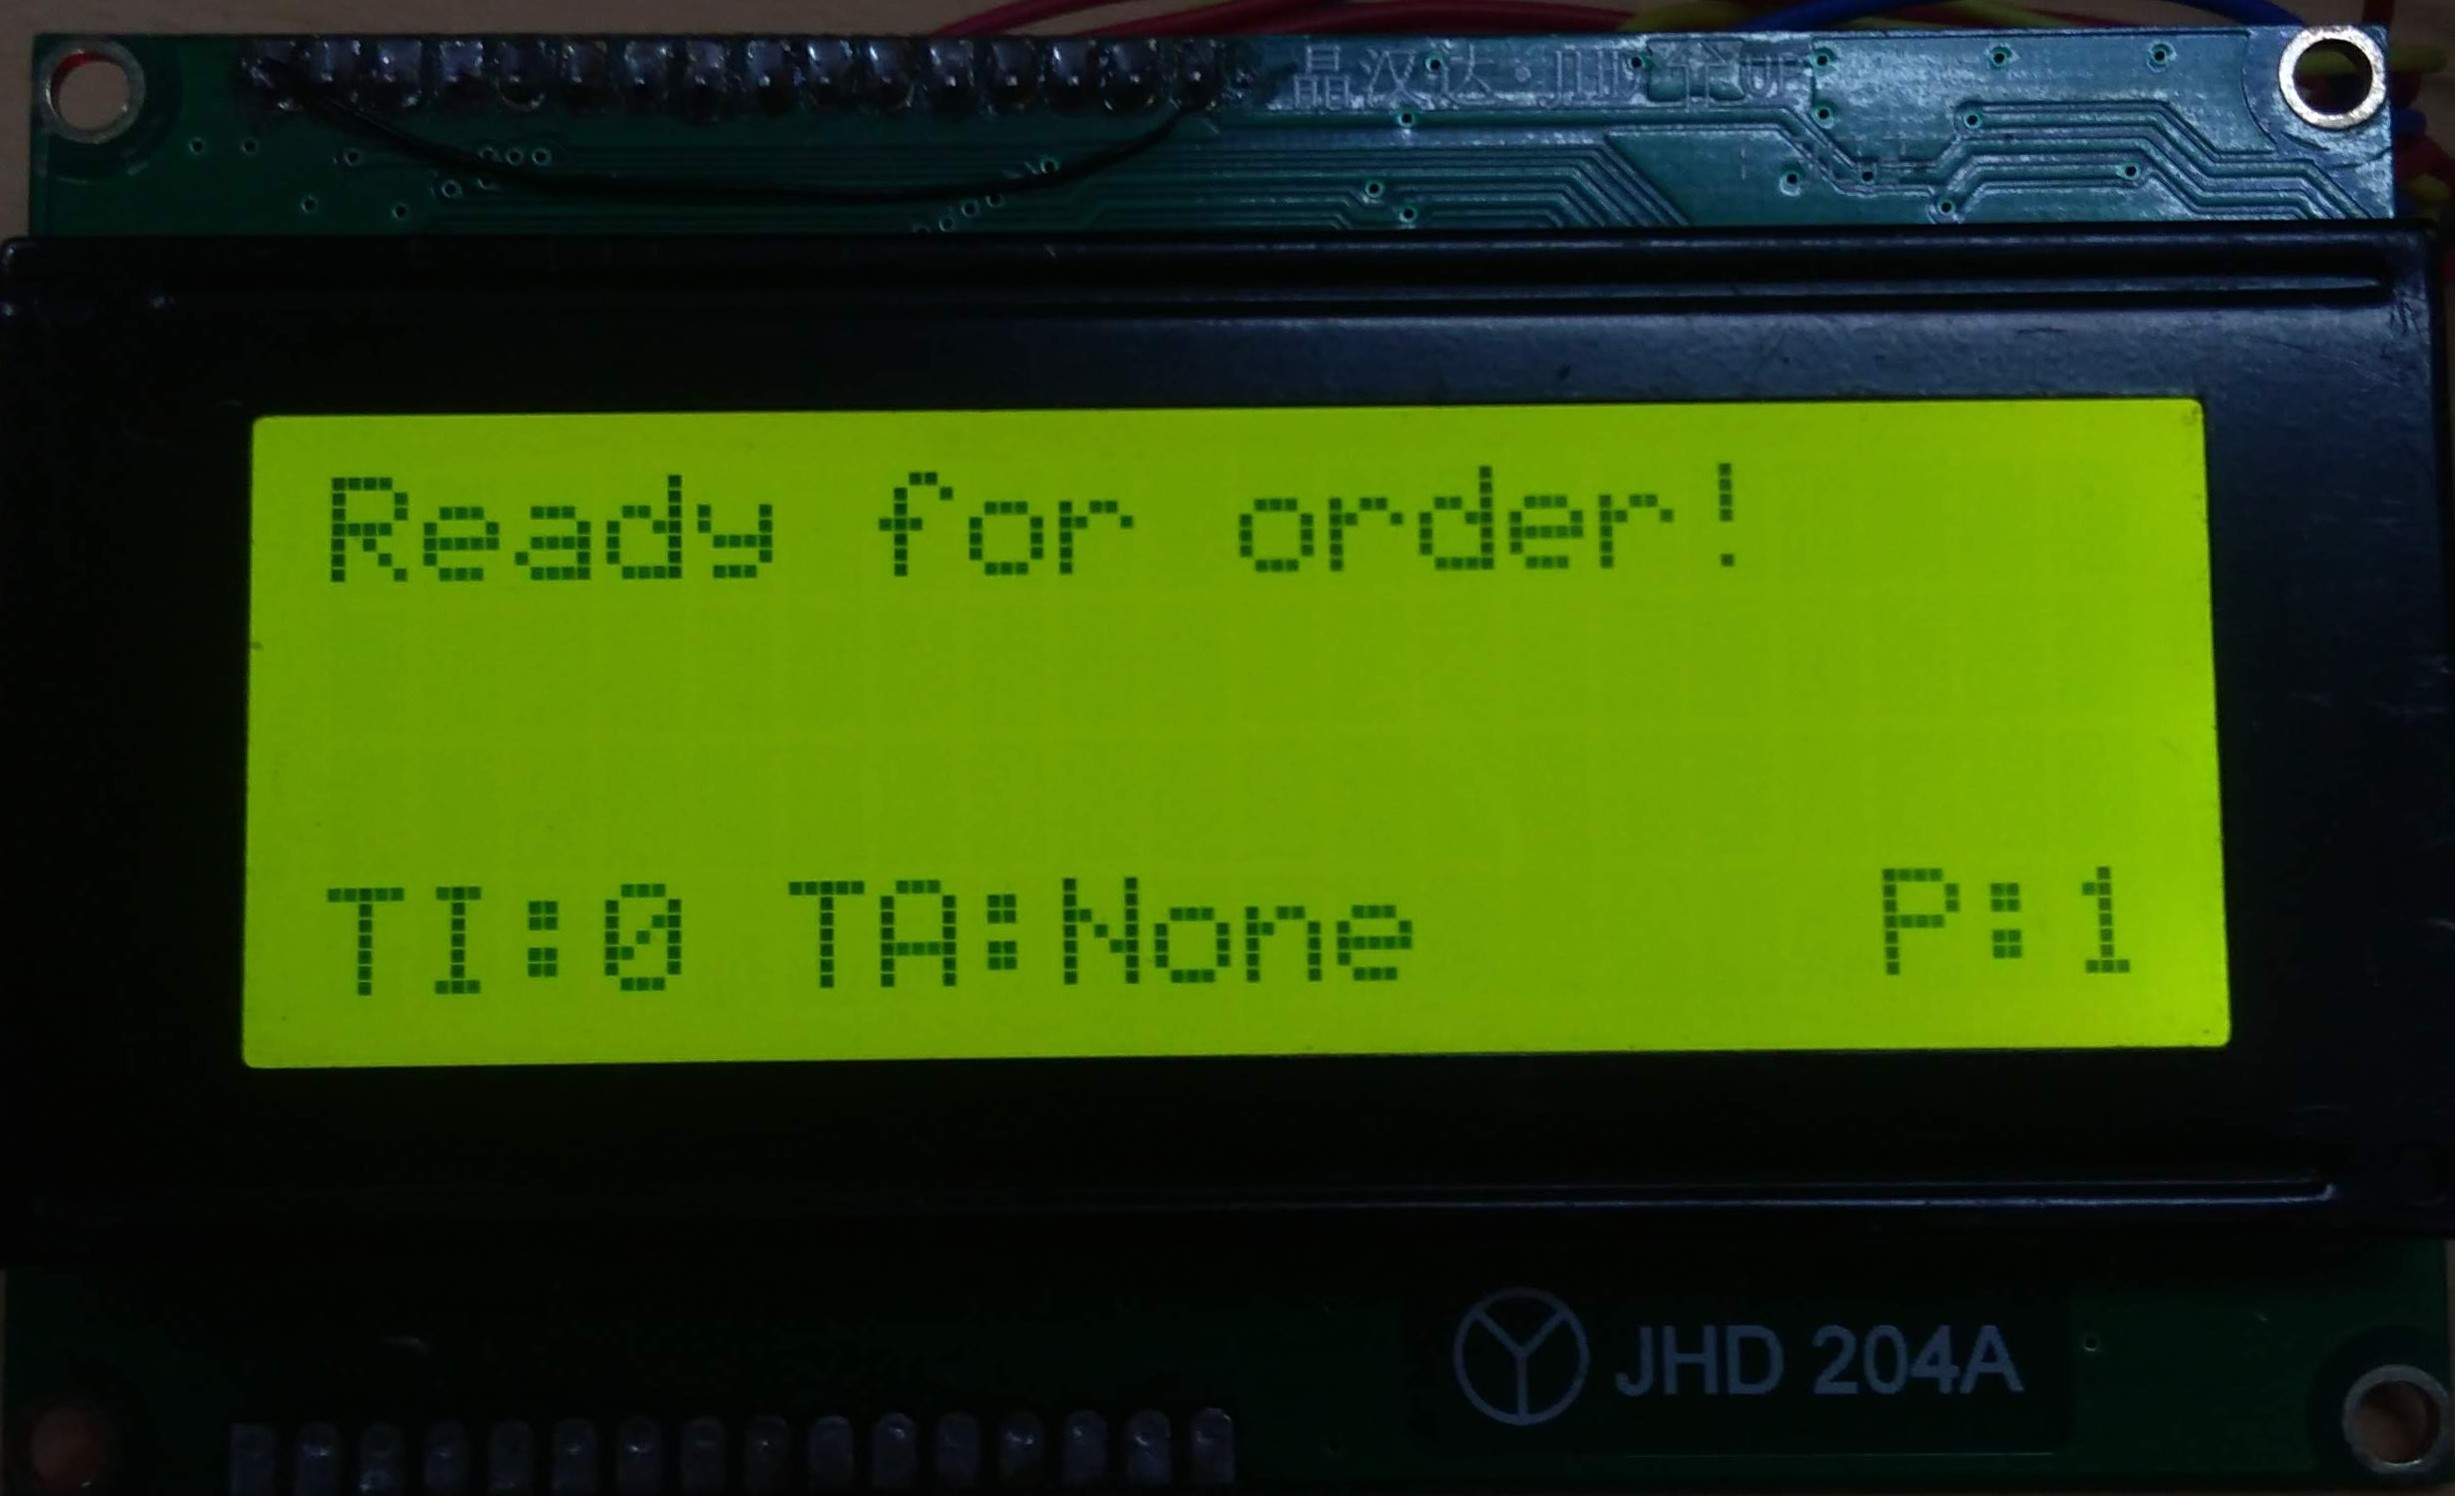
\includegraphics[width=1\textwidth]{ready}
		\end{subfigure}%
		\begin{subfigure}{.5\textwidth}
			\centering
			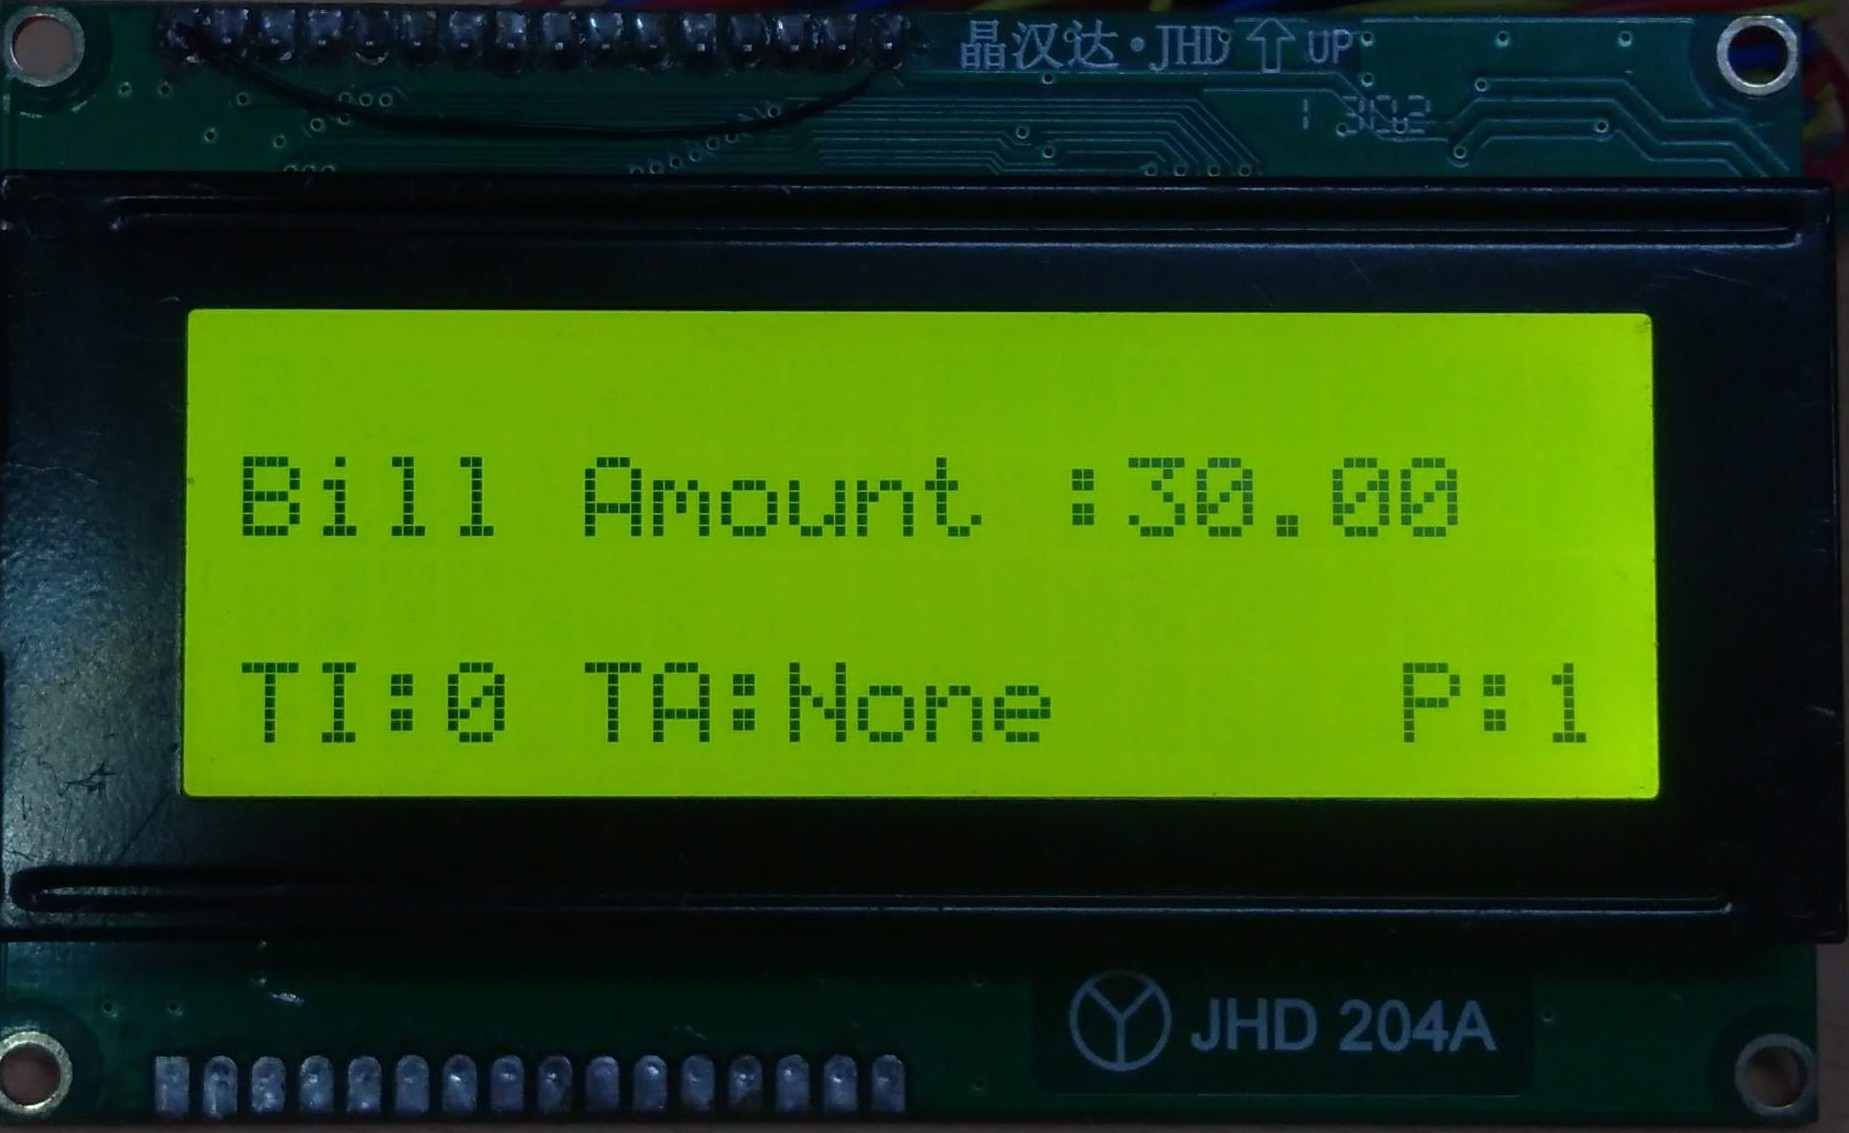
\includegraphics[width=1\textwidth]{bill_amount}
		\end{subfigure}
			\caption[short]{LCD Output}
		\end{figure}		    	
    \newpage
\subsection{MySQL Database Tables and Config File}
\begin{figure}[h]
	\centering
	\begin{subfigure}{.5\textwidth}
		\centering
		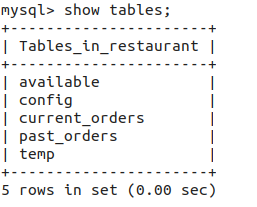
\includegraphics[width=.8\textwidth]{all_tables}
	\end{subfigure}%
	\begin{subfigure}{.5\textwidth}
		\centering
		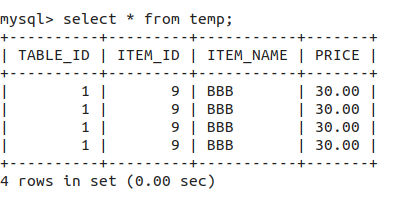
\includegraphics[width=1\textwidth]{temp_table}
	\end{subfigure}
	\begin{subfigure}{.5\textwidth}
		\centering
		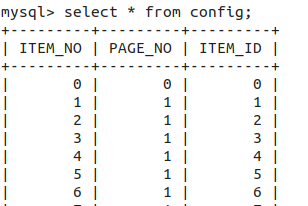
\includegraphics[width=0.8\textwidth]{config_table}
	\end{subfigure}%
	\begin{subfigure}{.5\textwidth}
		\centering
		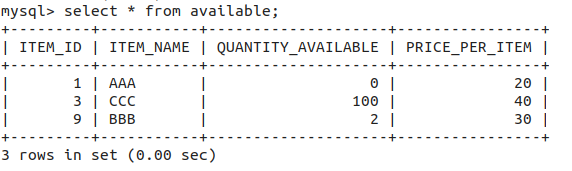
\includegraphics[width=1\textwidth]{available_table}
	\end{subfigure}
	\begin{subfigure}{.5\textwidth}
		\centering
		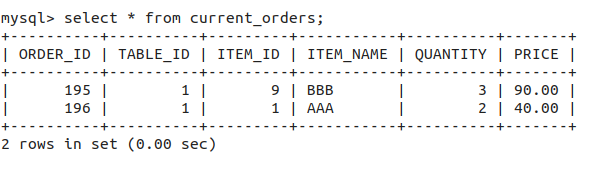
\includegraphics[width=0.8\textwidth]{current_orders}
	\end{subfigure}%
	\begin{subfigure}{.5\textwidth}
		\centering
		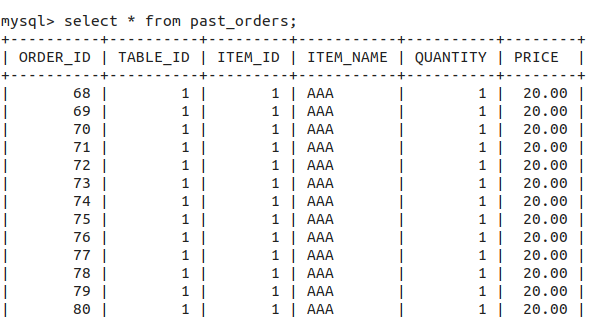
\includegraphics[width=1\textwidth]{past_orders}
	\end{subfigure}
	\caption[short]{MySQL Database Tables Created}
\end{figure}		    	
	    
	    

		

	\newpage
	\nocite{*}	
	\bibliographystyle{plain}
	\bibliography{report.bib}

\end{document}
